\documentclass[12pt]{article}

% Packages
\usepackage{amsmath, amssymb}
\usepackage{graphicx}
\usepackage{hyperref}
\usepackage{geometry}
\usepackage{fancyhdr}
\usepackage{float}

% Page layout
\geometry{a4paper, margin=1in}
\setlength{\parskip}{1em}
\setlength{\parindent}{0em}

% Header and Footer
\pagestyle{fancy}
\fancyhf{}
\fancyhead[L]{Steam Game Recommender System}
\fancyfoot[C]{\thepage}

\title{\textbf{Final Report : Steam Game Recommender System}}
\author{Zeyu Liang}
\date{\today}
\begin{document}
\maketitle
\section{Introduction}
The increasing size of game libraries on platforms like Steam makes it challenging for users to find games suited to their preferences. This project addresses this issue by building a recommendation system leveraging user interaction data, such as game reviews, playtime, and ratings. The goal of the project is to develop a model that accurately predicts and recommends games tailored to individual user preferences.

The project focuses on implementing collaborative filtering techniques alongside content-based approaches to ensure diverse and accurate recommendations.
\section{Methods and Approach}
\subsection{Data Collection and Preprocessing}
The dataset used for this project was sourced from publicly available Steam data from platforms Kaggle . Key preprocessing steps included:
\begin{itemize}
	\item \textbf{Data Cleaning}: Handling missing values, filtering out incomplete records, and ensuring data consistency.
	\item \textbf{Feature Engineering}: Encoding playtime and \texttt{is\_recommended} features from the original data into a single feature: rating.  Of course, whether the function I used to tranform playtime and \texttt{is\_recommended} to rating can be improved and argued. Please take a look at the \texttt{calculate\_rating} function in my code for more details. It's worth to note that I manually make a cut, give a rating 10.0(highest possible rating) when a user spends over 100 hours on a game and she likes the game, thus it's hard to distinguish how user would rate the game differently for 100 and 200 hours. Making the prediction non-linear for higher score. 
	\item \textbf{Data Transformation}: Splitting the dataset into training and testing sets for evaluation of the recommendation model. This process is actually meaningless as one can not test the model using the test data. This is because the model has to fill the hidden 100 features(parameters) for each user in \texttt{trainning\_data} and each game during the trainning process. But one can not guess the hidden features for test data. I will address this part later in the report.
\end{itemize}

\subsection{Model Development and Evaluation}
\begin{enumerate}
	\item \textbf{Collaborative Filtering}:
	\begin{itemize}
		\item \textbf{Matrix Factorization}: Singular Value Decomposition (SVD) was used to factorize the user-item interaction matrix into low-dimensional latent features. 
		\item \textbf{Prediction}: The predicted interaction score between a user and a game is computed as the dot product of the user's and game's latent features.
		\item \textbf{Game Recommendations}: Games with the highest similarity scores were recommended to users based on their historical interactions.
	\end{itemize}
	
	\item \textbf{Evaluation}:
	\begin{itemize}
		\item \textbf{Root Mean Square Error (RMSE)}: Used to evaluate the accuracy of predictions in collaborative filtering.
		\item \textbf{Regularization} : Included both \texttt{game\_features} and \texttt{user\_features} regularization terms to prevent overfitting. 
	\end{itemize}
\end{enumerate}

\section{Results and Analysis}
\subsection{Training Loss}
Due to a coding error that I made, I lost the initial training loss for first 100 iterations. Since training the model takes a very long time, I don't want to re-train the model to include the full data. As I remembered, the initial loss for iteration 1 is roughly $2*10^9$. After 400 iterations of training, the loss is about 264000. Shown in Figure 1.
\begin{figure}[h]
	\centering
	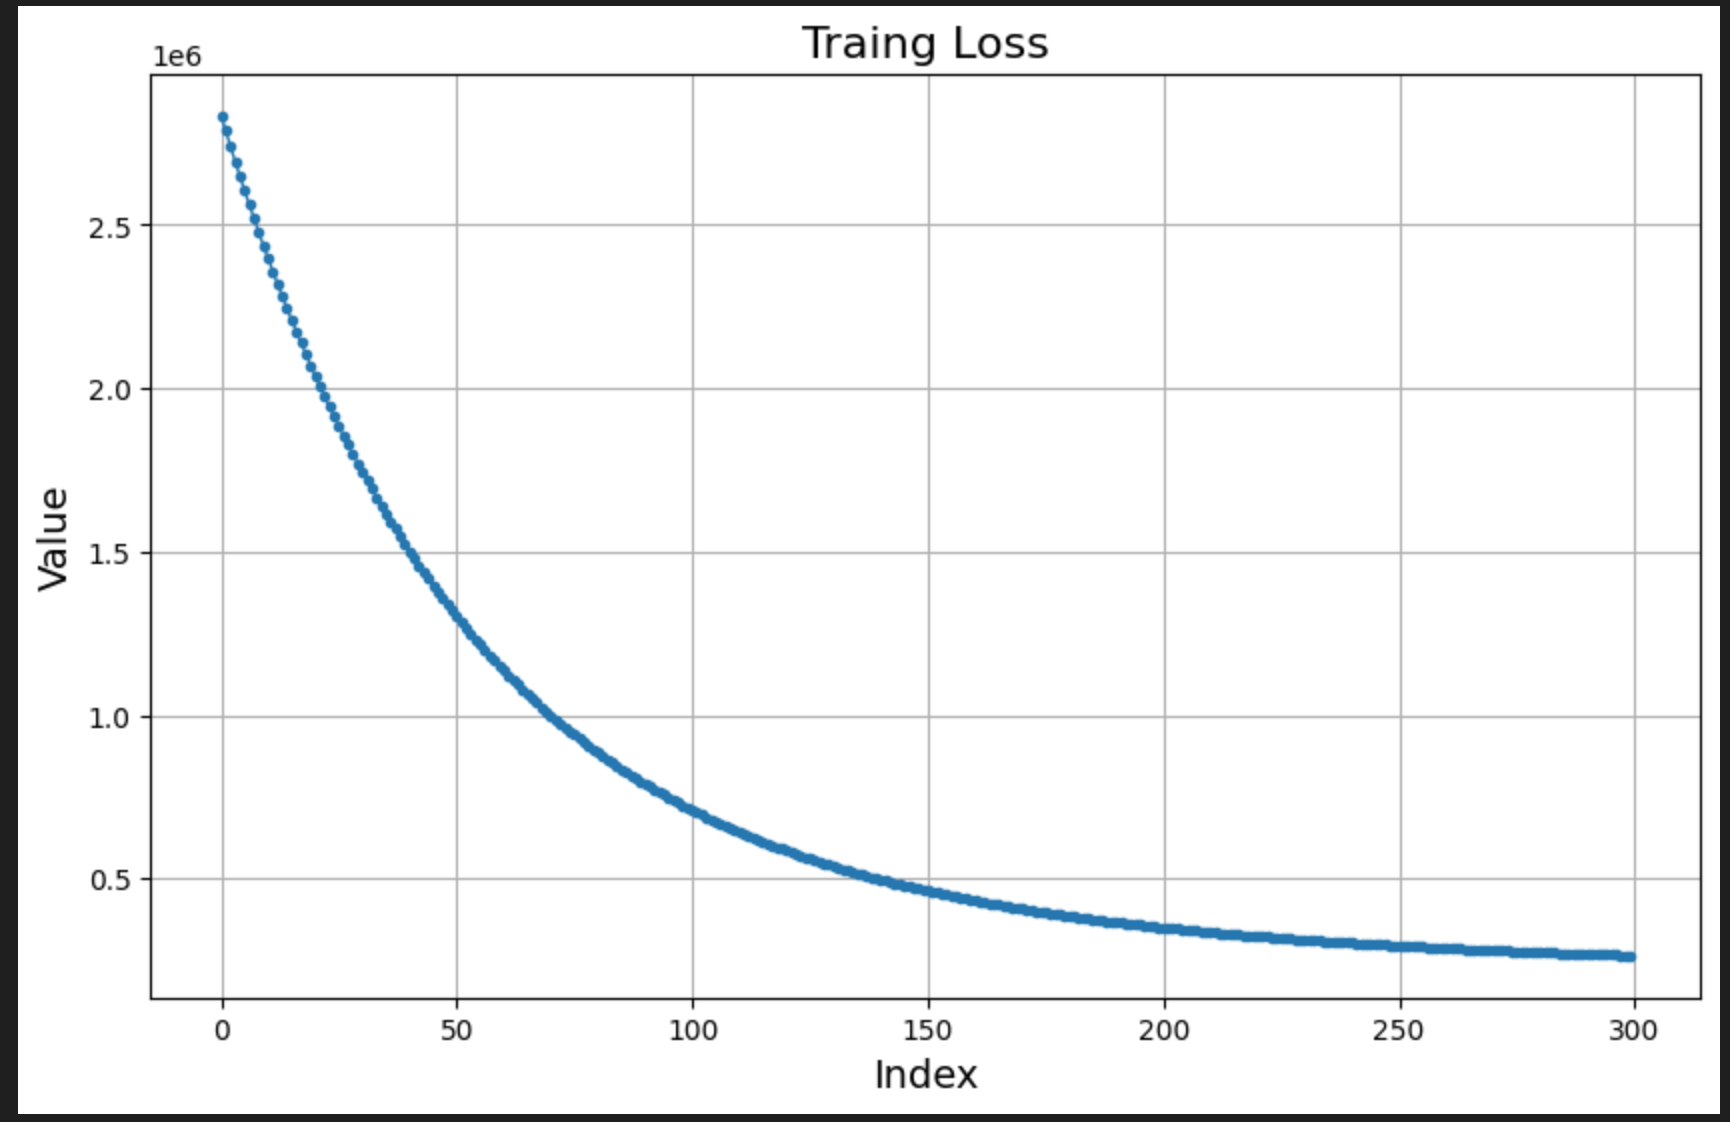
\includegraphics[width=0.8\textwidth]{loss.png} % Replace with your image file name
	\caption{Training Loss}
	\label{fig:Training Loss}
\end{figure}
\subsection{Comparison and Testing}
As shown in Figure 2, the model is not good at predicting very high score when a user has a close to 10 actual rating. I suspected the reason for this is that a 10 rating is not achieved by linear prediction, as explained earlier in 2.1 feature engineering.  Therefore, the model can not follow the normal rule to predict very high rating.
\begin{figure}[h]
	\centering
	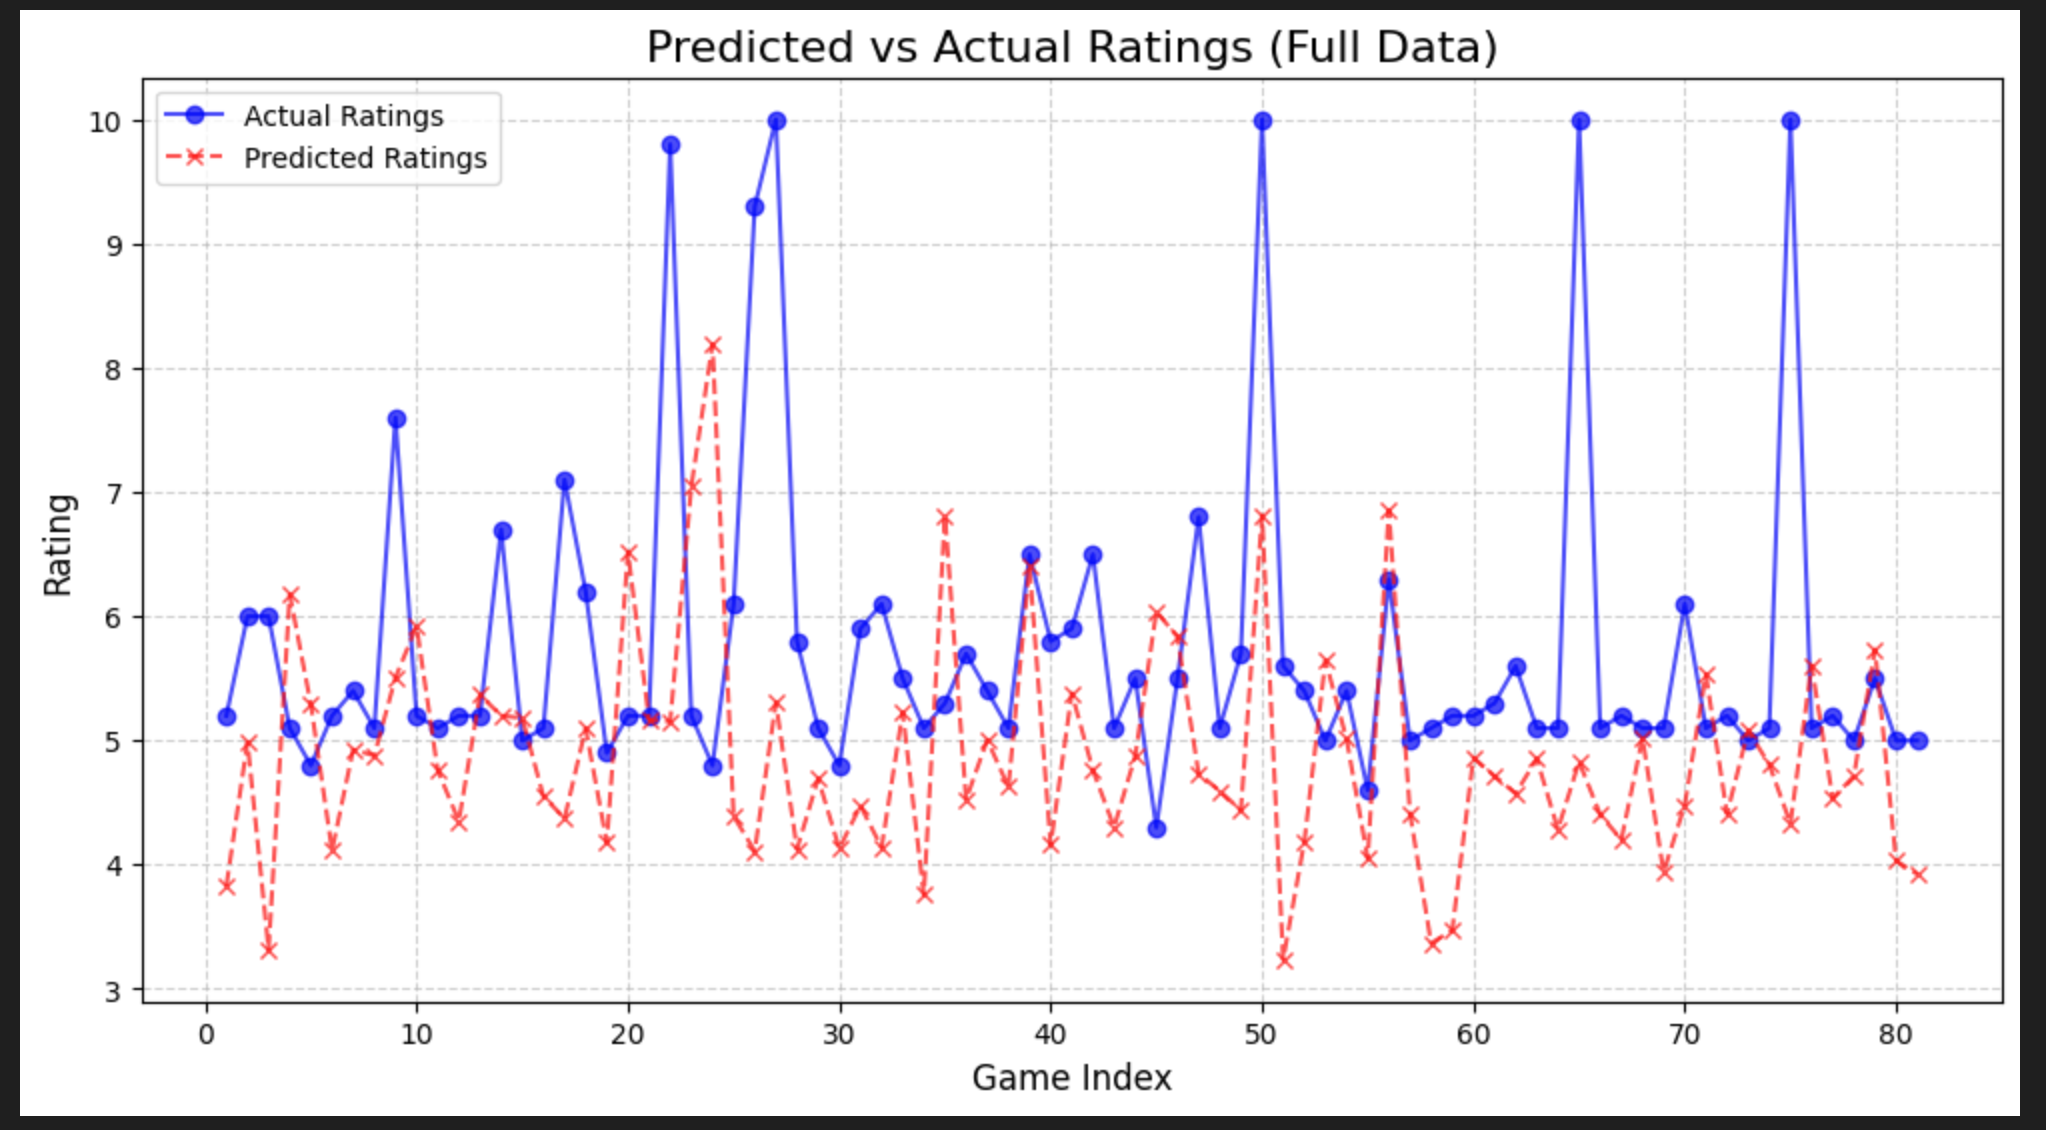
\includegraphics[width=0.8\textwidth]{compare.png} % Replace with your image file name
	\caption{Comparison for a random user}
	\label{fig:Comparison for a random user}
\end{figure}

\section{Conclusion and Reflection}
The developed Steam Game Recommender System effectively combines collaborative filtering and content-based techniques to provide personalized recommendations. 
\subsection{A Mistake}
At the beginning of this project, I mistakenly believed it was possible to select game features such as MOBA, 3D, RPG, adventure, etc., and train the model using these features. My idea was to assign each game a set of values reflecting its composition, such as Dota being 90 percent MOBA and 5 percent  3D, and to assign each user a parameter reflecting their preferences, such as User A enjoying 50 percent  MOBA games. This approach would allow the model to generate recommendations even for users with no prior history by enabling them to manually input their preferences for different game genres. However, I later realized that the features computed by the model are entirely abstract and not interpretable by humans. There is no way to directly map a specific feature parameter to a real-world attribute, which made it impossible to achieve the functionality I initially envisioned in my mid-term proposal. For the same reason, it is also not feasible to use test data to evaluate the model, as the users in the test data do not have assigned parameter features.
\subsection{Future Improvements}
Incorporate more features in the feature engineering part to generate the rating. For this project and the data I got from Kaggle, playtime and \texttt{is\_recommended} are the only useful two features I can use to produce a rating. Selecting more and relevant features from other source  can make the model fit the data better, and thus produce more accurate prediction. Moreover, I can  improve the function I used in compute rating. Making the rating to range from 0 to 100 rather than 0 to 10, and ensuring that  the prediction function remains linear. These improvements increase both the complexity and precision of the prediction function, thereby enabling the model to better capture the underlying patterns in the data.
\end{document}